\documentclass[10pt]{beamer} 
     \hypersetup{pdfpagemode=FullScreen} 
     \usepackage{tikz} 
     \usetikzlibrary{shadows,patterns,shapes} 
     \usetikzlibrary{shapes.arrows,chains} 
     % serifenfreier Font -- fuer Praesentation geeignet/er 
     \listfiles % damit im Log alle benutzten Pakete aufgelistet werden 
     \usetheme[progressbar=frametitle]{metropolis} 
     \usepackage{appendixnumberbeamer} 
     \usepackage{booktabs} 
     \usepackage[scale=2]{ccicons} 
     \usepackage[utf8]{inputenc} 
     \usepackage{pgfplots} 
     \usepgfplotslibrary{dateplot} 
     \usepackage[ngerman]{babel} 
     \usepackage{xspace} 
     \usebackgroundtemplate{
     \tikz[overlay,remember picture] 
     \node[opacity=0.3, at=(current page.south east),anchor=south east,inner sep=0pt] {
     
\includegraphics[width=100mm]{./PDFcreater/Pictures/background.png}};
     } 
     %\usebackgroundtemplate{
\includegraphics[,right]{./PDFcreater/Pictures/background.png}}
     \definecolor{Purple}{HTML}{6D087C}
     \definecolor{Orange}{HTML}{CF4A30}
     
     % Theme colors are derived from these two elements
     \setbeamercolor{alerted text}{fg=Orange}
     
     % ... however you can of course override styles of all elements 
     \setbeamercolor{frametitle}{bg=Purple}
     
     \title{SolidEdge Feedback der Studierenden} 
     \begin{document} 
     \maketitle 
\begin{frame}[fragile]{Benoetigte Stundenzahl vom gesamten CAD Kurs pro Woche} 
 \begin{figure}
 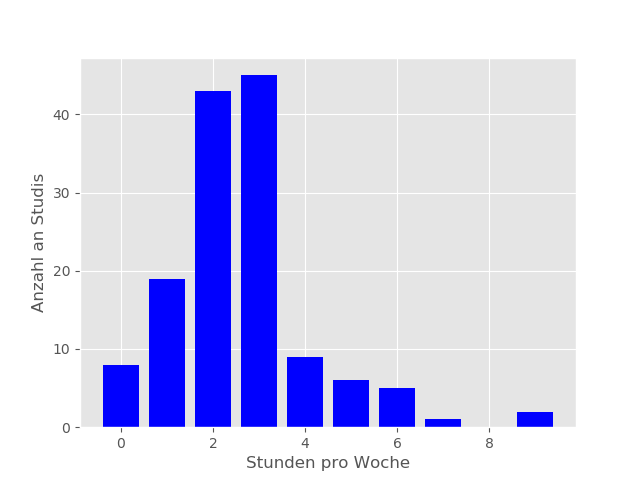
\includegraphics[width= 0.9\linewidth]{./PDFcreater/Plots/Benoetigte+Stundenzahl+vom+gesamten+CAD+Kurs+pro+Woche.png};
 \end{figure}
 \end{frame}
\begin{frame}[fragile]{Der Lehrinhalt war ausreichend um die HA zu bearbeiten} 
 \begin{figure}
 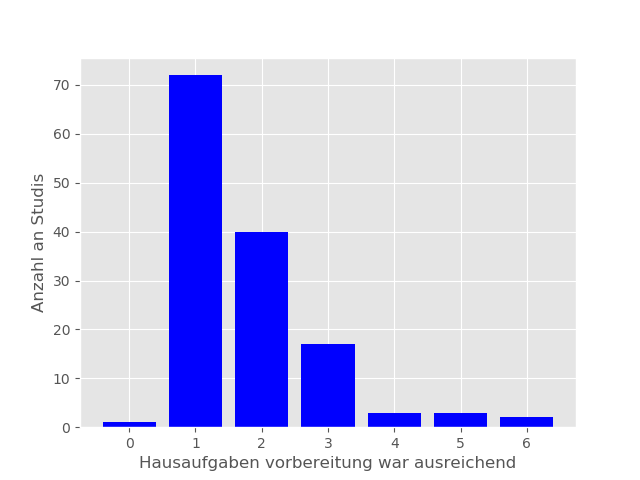
\includegraphics[width= 0.9\linewidth]{./PDFcreater/Plots/Der+Lehrinhalt+war+ausreichend+um+die+HA+zu+bearbeiten.png};
 \end{figure}
 \end{frame}
\begin{frame}[fragile]{Der Schwierigkeitsgrad war hoch} 
 \begin{figure}
 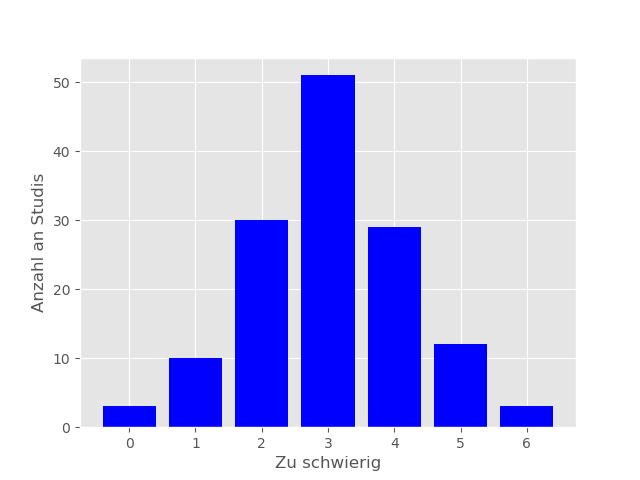
\includegraphics[width= 0.9\linewidth]{./PDFcreater/Plots/Der+Schwierigkeitsgrad+war+hoch.png};
 \end{figure}
 \end{frame}
\begin{frame}[fragile]{Die Formulierungen in der Hausaufgabe waren eindeutig} 
 \begin{figure}
 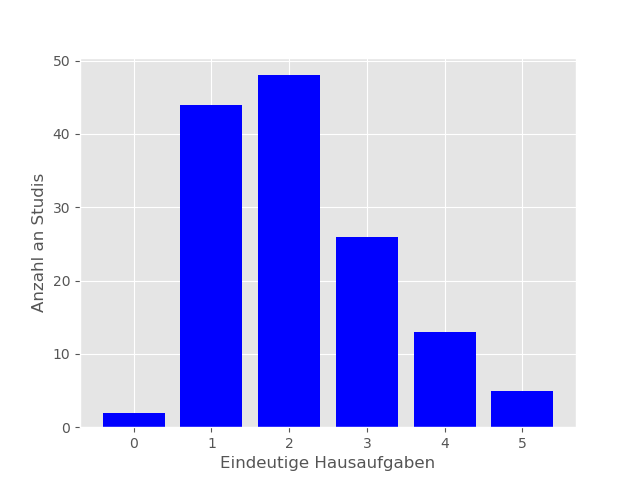
\includegraphics[width= 0.9\linewidth]{./PDFcreater/Plots/Die+Formulierungen+in+der+Hausaufgabe+waren+eindeutig.png};
 \end{figure}
 \end{frame}
\begin{frame}[fragile]{Die Hausaufgabe sollte vom Umfang her reduziert werden} 
 \begin{figure}
 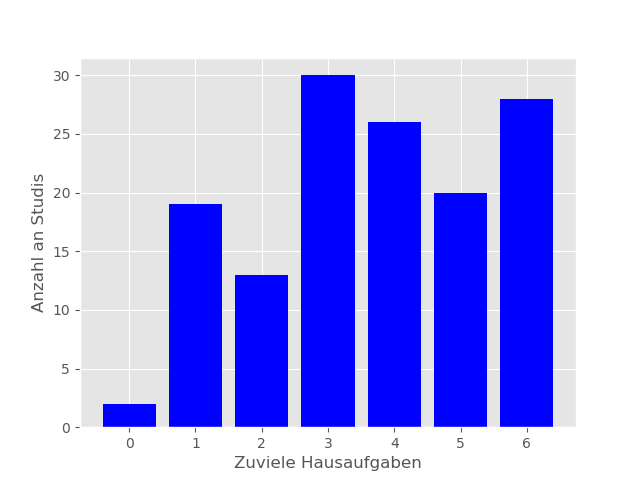
\includegraphics[width= 0.9\linewidth]{./PDFcreater/Plots/Die+Hausaufgabe+sollte+vom+Umfang+her+reduziert+werden.png};
 \end{figure}
 \end{frame}
\begin{frame}[fragile]{Die Uebungen sind gut strukturiert} 
 \begin{figure}
 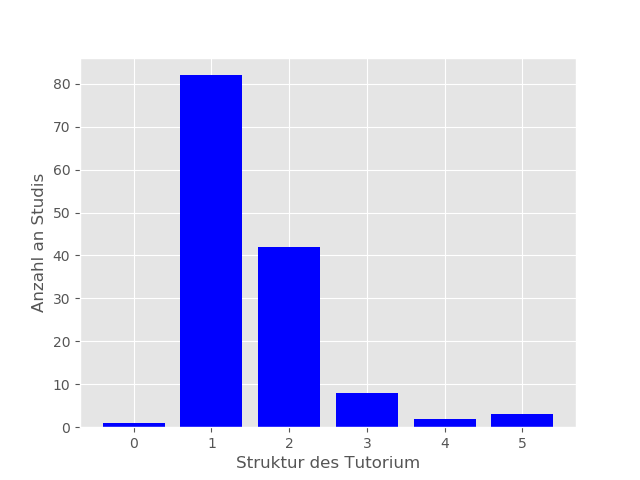
\includegraphics[width= 0.9\linewidth]{./PDFcreater/Plots/Die+Uebungen+sind+gut+strukturiert.png};
 \end{figure}
 \end{frame}
\begin{frame}[fragile]{Die Uebungsbeispiele sind gut gewaehlt} 
 \begin{figure}
 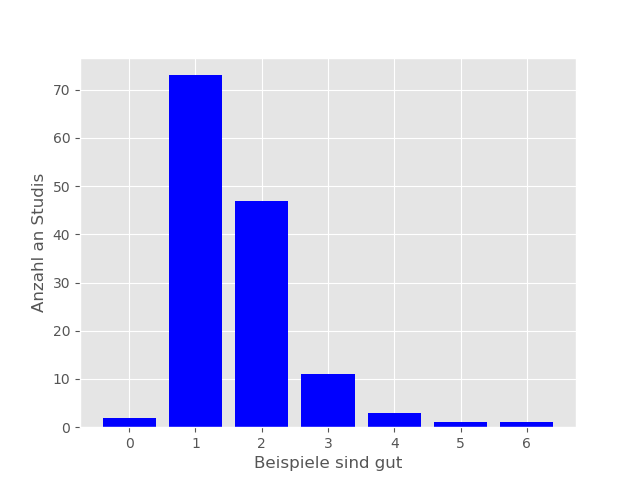
\includegraphics[width= 0.9\linewidth]{./PDFcreater/Plots/Die+Uebungsbeispiele+sind+gut+gewaehlt.png};
 \end{figure}
 \end{frame}
\begin{frame}[fragile]{Geschlecht der Studis} 
 \begin{figure}
 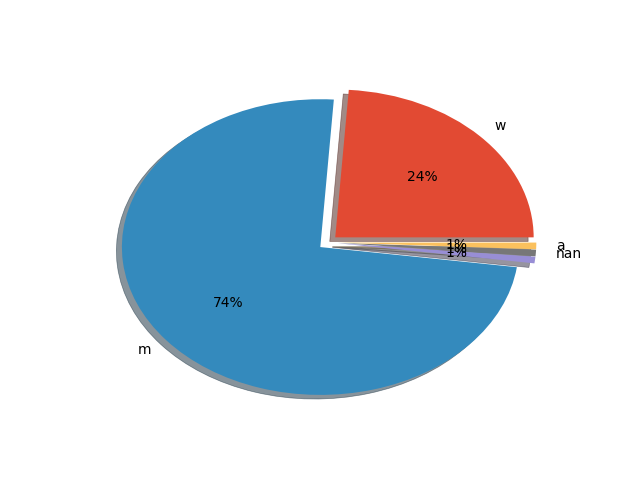
\includegraphics[width= 0.9\linewidth]{./PDFcreater/Plots/Geschlecht+der+Studis.png};
 \end{figure}
 \end{frame}
\begin{frame}[fragile]{Ich habe die Uebungsaufgaben alle gemacht} 
 \begin{figure}
 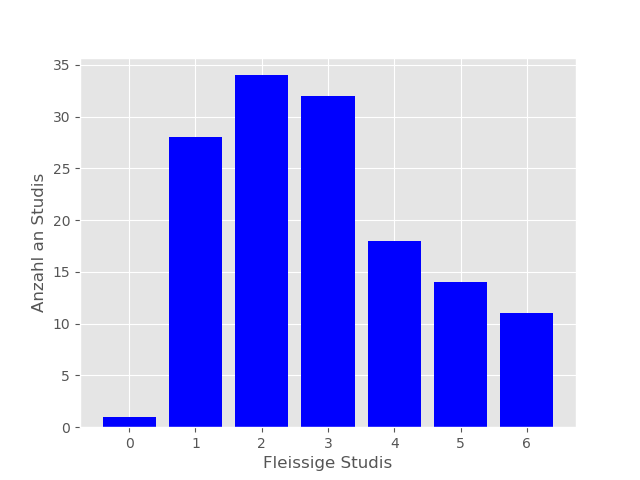
\includegraphics[width= 0.9\linewidth]{./PDFcreater/Plots/Ich+habe+die+Uebungsaufgaben+alle+gemacht.png};
 \end{figure}
 \end{frame}
\begin{frame}[fragile]{Ich habe mich schon fruehzeitig mit dem Programm zu Hause beschaeftigt} 
 \begin{figure}
 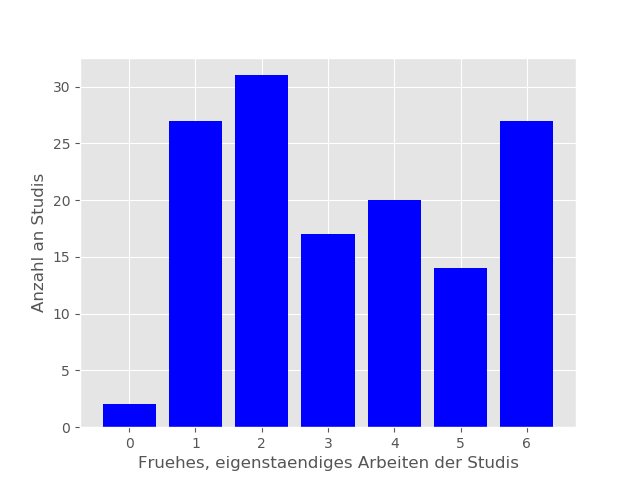
\includegraphics[width= 0.9\linewidth]{./PDFcreater/Plots/Ich+habe+mich+schon+fruehzeitig+mit+dem+Programm+zu+Hause+beschaeftigt.png};
 \end{figure}
 \end{frame}
\begin{frame}[fragile]{Ich habe viel Zeit zur Bearbeitung der Hausaufgabe benoetigt} 
 \begin{figure}
 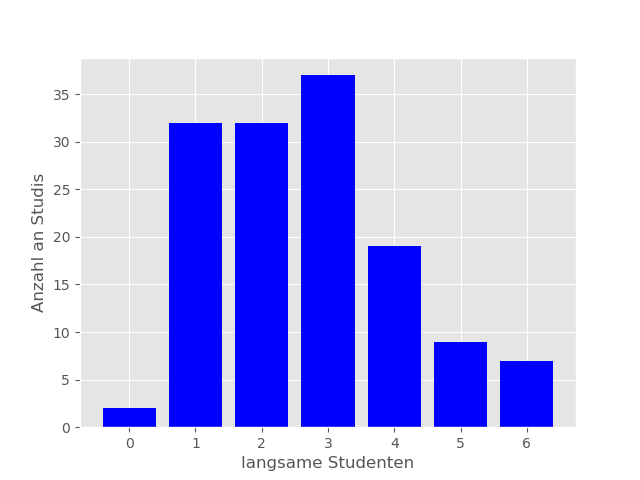
\includegraphics[width= 0.9\linewidth]{./PDFcreater/Plots/Ich+habe+viel+Zeit+zur+Bearbeitung+der+Hausaufgabe+benoetigt.png};
 \end{figure}
 \end{frame}
\begin{frame}[fragile]{Ich haette gerne mehr Uebungsaufgaben gehabt} 
 \begin{figure}
 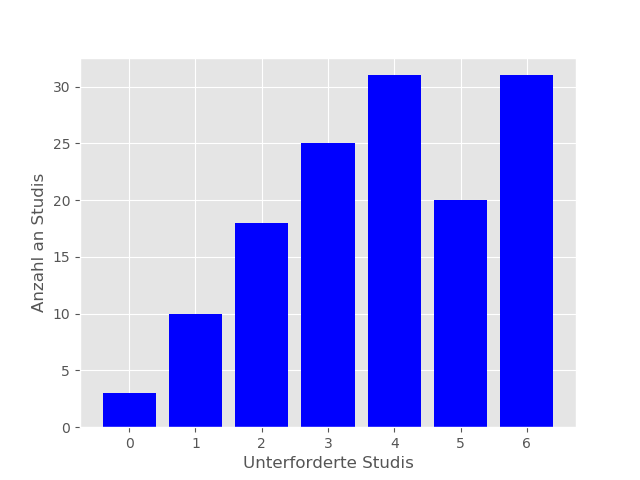
\includegraphics[width= 0.9\linewidth]{./PDFcreater/Plots/Ich+haette+gerne+mehr+Uebungsaufgaben+gehabt.png};
 \end{figure}
 \end{frame}
\begin{frame}[fragile]{Ich war immer gut auf das Tutorium vorbereitet} 
 \begin{figure}
 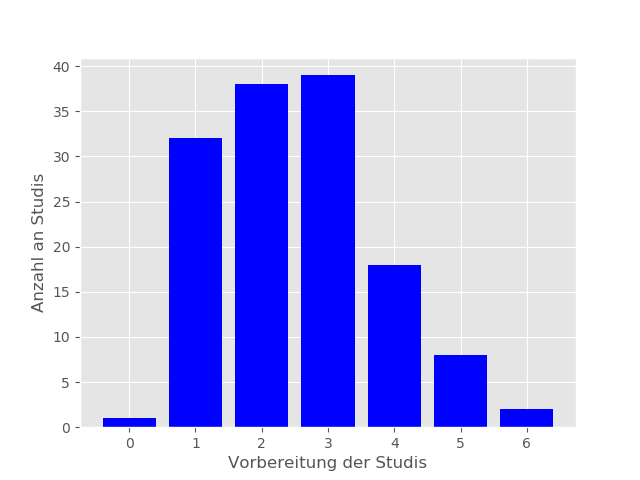
\includegraphics[width= 0.9\linewidth]{./PDFcreater/Plots/Ich+war+immer+gut+auf+das+Tutorium+vorbereitet.png};
 \end{figure}
 \end{frame}
\begin{frame}[fragile]{Semester der Studierenden} 
 \begin{figure}
 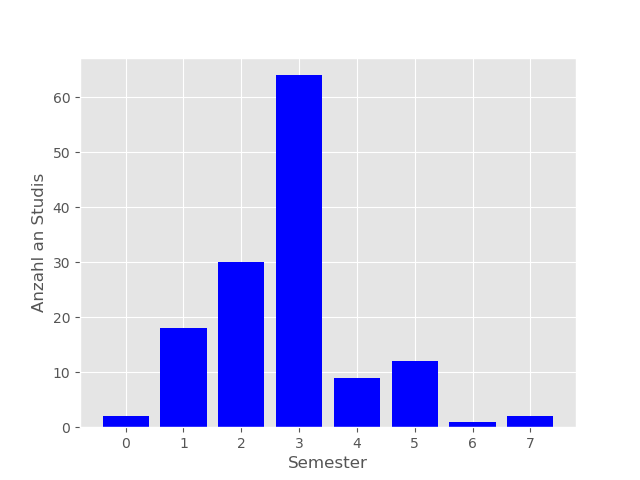
\includegraphics[width= 0.9\linewidth]{./PDFcreater/Plots/Semester+der+Studierenden.png};
 \end{figure}
 \end{frame}
\begin{frame}[fragile]{Studiengang der Studis} 
 \begin{figure}
 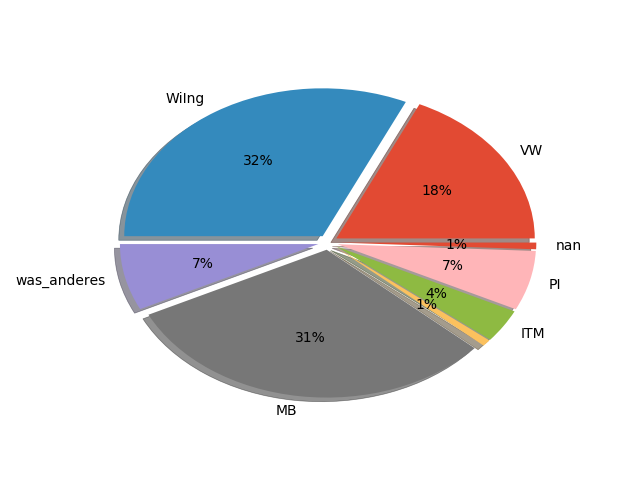
\includegraphics[width= 0.9\linewidth]{./PDFcreater/Plots/Studiengang+der+Studis.png};
 \end{figure}
 \end{frame}
\begin{frame}[fragile]{Tutor der Studis} 
 \begin{figure}
 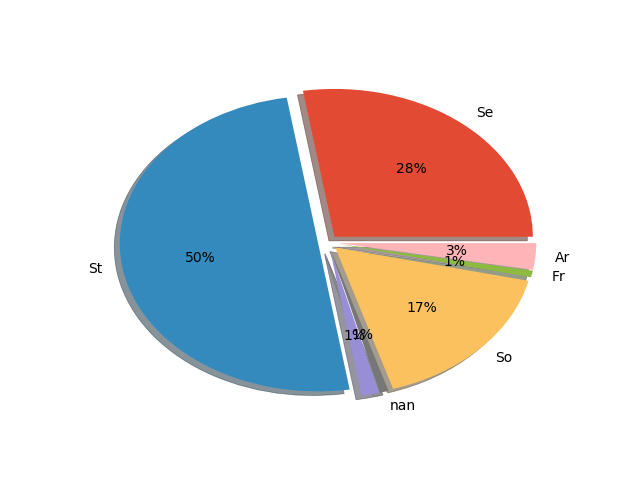
\includegraphics[width= 0.9\linewidth]{./PDFcreater/Plots/Tutor+der+Studis.png};
 \end{figure}
 \end{frame}
\begin{frame}[fragile]{Tutor foerdert aktive Teilnahme der Studenten} 
 \begin{figure}
 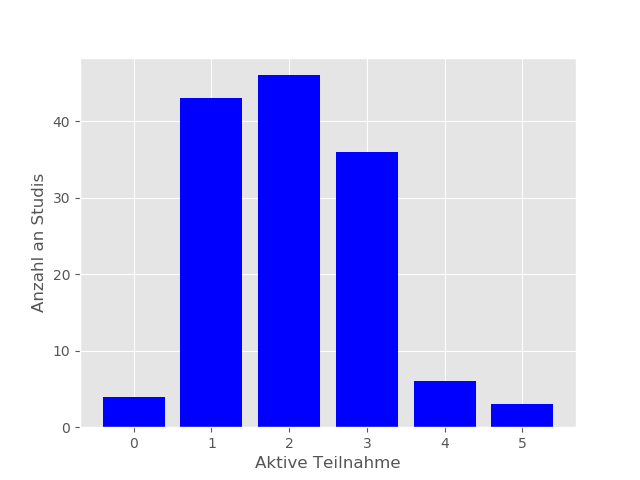
\includegraphics[width= 0.9\linewidth]{./PDFcreater/Plots/Tutor+foerdert+aktive+Teilnahme+der+Studenten.png};
 \end{figure}
 \end{frame}
\begin{frame}[fragile]{Tutor ist immer gut auf das Tutorium vorbereitet} 
 \begin{figure}
 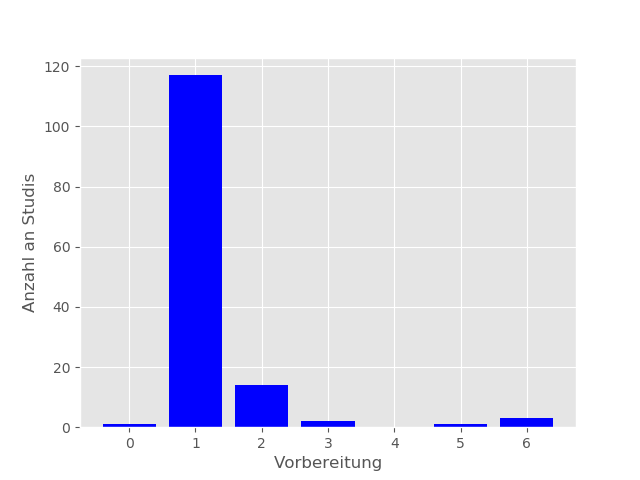
\includegraphics[width= 0.9\linewidth]{./PDFcreater/Plots/Tutor+ist+immer+gut+auf+das+Tutorium+vorbereitet.png};
 \end{figure}
 \end{frame}
\begin{frame}[fragile]{Tutor kann den Lehrinhalt verstaendlich darlegen} 
 \begin{figure}
 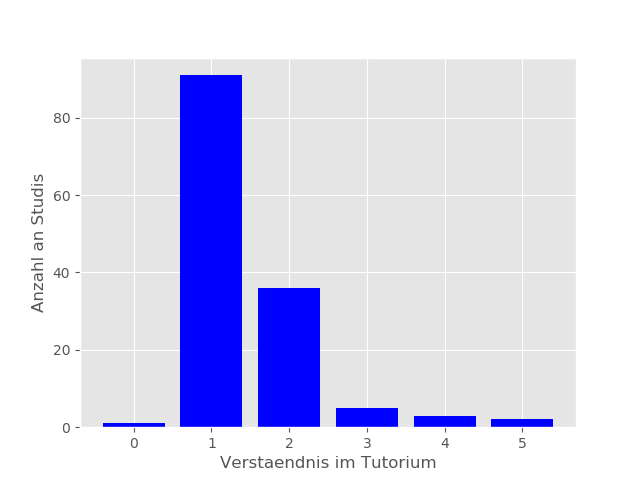
\includegraphics[width= 0.9\linewidth]{./PDFcreater/Plots/Tutor+kann+den+Lehrinhalt+verstaendlich+darlegen.png};
 \end{figure}
 \end{frame}
\end{document}